\documentclass[msc,numbers]{coppe}
\usepackage{amsmath,amssymb}
\usepackage{hyperref}
\usepackage{algpseudocode}
\usepackage{algorithm}

\makelosymbols
\makeloabbreviations

\begin{document}
    \title{Change Point Detection in End-to-End Measurements Time Series}
    \foreigntitle{Change Point Detection in End-to-End Measurements Time Series}
    \author{Diego}{Ximenes Mendes}
    \advisor{Prof.}{Edmundo}{Albuquerque de Souza e Silva}{Ph.D.}
  
    %\examiner{Prof.}{Nome do Primeiro Examinador Sobrenome}{D.Sc.}
    %\examiner{Prof.}{Nome do Segundo Examinador Sobrenome}{Ph.D.}
    %\examiner{Prof.}{Nome do Terceiro Examinador Sobrenome}{D.Sc.}
    %\examiner{Prof.}{Nome do Quarto Examinador Sobrenome}{Ph.D.}
    %\examiner{Prof.}{Nome do Quinto Examinador Sobrenome}{Ph.D.}
    \department{PESC}
    \date{01}{2017}
  
    \keyword{Change Point Detection}
    \keyword{Time Series}
    \keyword{Machine Learning}
  
    \maketitle
  
    \frontmatter
    %\dedication{A algu\'em cujo valor \'e digno desta dedicat\'oria.}
  
    %\chapter*{Agradecimentos}
  
    \begin{abstract}
    To better understand the performance of it's own network, a major
Tier-3 Brazilian ISP, in partnership with UFRJ and the startup TGR,
established a project to monitor the service provided to a subset
of it's customers.

In this context, guided by the specific ISP's network's charateristics
and the current measurement process,
this dissertation aims to check the viability of
only using end-to-end QoS measures, and traceroutes,
to identify and localize network events. An event can be interpreted as a
behavioral change in a network equipment, that affect the quality of service
perceived by the end-users,
such as a router failure. The localization procedure defines a set of
feasible locations where the event could have happened.

For such purpose, this work proposes a data analytics framework, which is able
to track statistical changes in the QoS time series of different
clients.
To detect and localize events, the mechanism correlates these modification
patterns with traceroutes.
In order to increase the system's performance,
this dissertation also indicates possible improvements in the current
measurement methodology.

    \end{abstract}
  
    \begin{foreignabstract}
    To better understand the performance of it's own network, a major
Tier-3 Brazilian ISP, in partnership with UFRJ and the startup TGR,
established a project to monitor the service provided to a subset
of it's customers.

In this context, guided by the specific ISP's network's charateristics
and the current measurement process,
this dissertation aims to check the viability of
only using end-to-end QoS measures, and traceroutes,
to identify and localize network events. An event can be interpreted as a
behavioral change in a network equipment, that affect the quality of service
perceived by the end-users,
such as a router failure. The localization procedure defines a set of
feasible locations where the event could have happened.

For such purpose, this work proposes a data analytics framework, which is able
to track statistical changes in the QoS time series of different
clients.
To detect and localize events, the mechanism correlates these modification
patterns with traceroutes.
In order to increase the system's performance,
this dissertation also indicates possible improvements in the current
measurement methodology.

    \end{foreignabstract}
  
    \tableofcontents
    \listoffigures
    \listoftables
    \printlosymbols
    \printloabbreviations
  
    \mainmatter
  
    \chapter{Introduction}

To better understand the performance of it's own network, a major
tier-3 Brazilian \gls*{isp}, in partnership with \gls*{ufrj} and a startup
incubated at this university,
established a project to monitor the service provided to a subset
of it's customers.

Considering the \gls*{isp}'s cable-television infrastructure,
which runs \gls*{docsis},
\gls*{qos} metrics are gathered through a software placed at home routers
connected to cable modems. This software is responsible to perform end-to-end
measurements against servers strategically located by the \gls*{isp}.

In this context, guided by the specific \gls*{isp}'s network's characteristics,
and the current measurement process,
this dissertation aims to check the viability of
only using end-to-end \gls*{qos} measures, and traceroutes,
to identify and localize network events. An event can be interpreted as a
behavioral change in a network equipment, that affect the quality of service
perceived by the end-users,
such as a router failure. The localization procedure defines a set of
feasible locations where the event could have happened.

For such purpose, this work proposes a data analytics framework, which is able
to track statistical changes in the \gls*{qos} time series of different
clients.
To detect and localize events, the mechanism correlates these modification
patterns with traceroutes.
In order to increase the system's performance,
this dissertation also indicates possible improvements in the current
measurement methodology.

\section{Contributions}

Considering the specific \gls*{isp}'s network topology,
and the already implemented
measurement process, next is listed this dissertation's main contributions.

\begin{itemize}
\item
A data analytics procedure, that only uses the available end-to-end \gls*{qos}
measurements, and traceroutes, to detect and localize network events.

\item
A list of possible improvements in the measurement methodology currently
employed by the startup, in order to enhance the proposed system's performance.

\end{itemize}

\section{Dissertation Outline}

Chapter~\ref{chap:literature_review} consists of a literature review, that
describes three previous systems that use
end-to-end measurements to localize network events.
To track statistical changes in the time series, the current
work deploys change point detection methods. Then,
Chapter~\ref{chap:change_point_detection} presents several of these algorithms,
including the developed strategies to better handle the end-to-end \gls*{qos} data
characteristics.
In Chapter~\ref{chap:methodology} is detailed the measurement methodology and
the proposed data analytics workflow.
Chapter~\ref{chap:results} presents several results when the proposed pipeline
was applied to real data.
Finally, Chapter~\ref{chap:conclusion} concludes the work and
points future directions.

The code developed to support this dissertation is available at
\url{https://bitbucket.org/diegoximenes/master_thesis}.
Unfortunately, due to a \gls*{nda},
the data used in this project can not be open sourced.

    \chapter{Literature Review of Change Point Detection} 

- Here the change point problem will be "defined", including offline and online versions.
- we deal with univariate unevenly time series. Explain that some methods can be expanded no multivariate
- unknow number of change points
- we disconsider changes in periodicity

\section{Notation}

In this work an univariate time series composed of $n$ points is defined by two vectors: $\mathbf{x} = (x_{1}, ..., x_{n})$ and $\mathbf{y} = (y_{1}, ..., y_{n})$. The value $y_{i}$ indicates the $i-$th sampled value and $x_{i}$ indicates the associated sample time. It is assumed that the points are sorted by time, that is, $x_{i - 1} < x_{i}$ for $i = 1, ..., n$. Since we consider unevenly time series $x_{i} - x_{i - 1}$ can be different for different $i$ values. For $s \ge t$ the following convention is adopted $\mathbf{y}_{s:t} = (y_{s}, ..., y_{t})$.

The presence of $k$ change points indicates that the data is splitted into $k+1$ segments, also called windows. Let $\tau_{i}$ indicate the $i-$th change point for $i=1,...,k$. Let $\tau_{0} = 0$ and $\tau_{k + 1} = n$. Then, the $i-$th segment is defined by $\mathbf{y}_{\tau_{i - 1} + 1 : \tau_{i}}$, assuming that $\tau_{i - 1} < \tau_{i}$ for $i = 0, ..., k + 1$. Therefore $\boldsymbol \tau = (\tau_{0}, ..., \tau_{k + 1})$.

\section{Sliding Window Techniques}

Mainly a change point detection algorithm aim to find $k$ and $\boldsymbol \tau$.

Describe sliding window techniques in change point detection. Describe how two windows can be compared. Probably this technique will not be part of my solution, but I will write about it since is the simplest and most intuitive solution.

\section{Combinatorial Optimization Model}  

\subsection{Constrained Case}

Given a fixed value of $k$, one approach is to define a cost function that measure the homogeneity of a segment and therefore choose the change points that globally optimize this homogeneity. Let the cost of the $i$-th segment be defined as $C(y_{\tau_{i - 1} + 1 : \tau_{i}})$. The cost of a segmentation is then $\sum \limits_{i = 1}^{k + 1} C(y_{\tau_{i - 1} + 1 : \tau_{i}})$.

A commom choice for function $C$ is the MSE (Mean Squared Error) which can capture changes in the mean. Another usual approach is to consider a distributin model and use the negative maximum log-likelihood. The latter can capture changes in mean and variance, also considers that data within a segment is iid. Therefore, given a fixed $k$, the optimal segmentation is obtained through the following optimization problem: 

\begin{equation}
    F_{k, n} = \min_{\boldsymbol \tau_{1 : k}} \sum \limits_{i = 1}^{k + 1} C(y_{\tau_{i - 1} + 1 : \tau_{i}})
\end{equation}

This problem can be solved using dynamic programming:

\begin{equation}
    F_{k, t} = 
    \begin{cases}
        0, & \text{if } k = 0 \text{ and } t = 0 \\
        \infty, & \text{if } k = 0 \text{ and } t > 0 \\
        \displaystyle \min_{s \in \{0, ..., t - 1\}} \left[ F_{k - 1, s} + C(y_{s + 1 : t}) \right], & \text{ otherwise}
    \end{cases}
\end{equation}

Given that function $C$ can be evaluated in $O(1)$, the overal time complexity of this algorithm is $O(k n^2)$.

\subsection{Segment Cost Function}

Several segment cost functions can be evaluated in $O(1)$ after a preprocessing phase. Next is provided the procedures to achieve this efficiency using MSE, negative maximum log-likelihood of normal and exponential distributions.

\subsubsection{MSE}

Let $\mu_{s, t}$ the mean value of the segment $\mathbf{y}_{s : t}$:

\begin{equation}
    \mu_{s, t} = \frac{\sum \limits_{i = s}^{t} y_{i}}{t - s + 1}
\end{equation}

Then, the $MSE(\mathbf{y}_{s : t})$ is defined as:

\begin{equation}
    \begin{aligned}
        MSE(\mathbf{y}_{s : t}) = \frac{\sum \limits_{i = s}^{t} (y_{i} - \mu_{s, t})^{2}}{t - s + 1} \\
        = \frac{\sum \limits_{i = s}^{t} (y_{i}^{2} - 2 y_{i} \mu_{s, t} + \mu_{s, t}^{2})}{t - s + 1} \\
        = \frac{\sum \limits_{i = s}^{t} y_{i}^{2} - 2 \mu_{s, t} \sum \limits_{i = s}^{t} y_{i} + (t - s + 1) \mu_{s, t}^{2}}{t - s + 1} \\
    \end{aligned}
\end{equation}

Let $S_{i} = \sum \limits_{j = 0}^{i} y_{j}$, that is, $\mathbf{S}$ represents the prefix sum of $\mathbf{y}$ for different indexes. $\mathbf{S}$ can be computed in $O(n)$ with the following dynamic programming procedure: 

\begin{equation}
    S_{i} = 
    \begin{cases}
        0, & \text{if } i = 0 \\
        S_{i - 1} + y_{i}, & \text{otherwise}
    \end{cases}
\end{equation}

Let $Q_{i} = \sum \limits_{j = 0}^{i} y_{j}^{2}$. As with $\mathbf{S}$, $\mathbf{Q}$ can be computed in $O(n)$: 

\begin{equation}
    Q_{i} = 
    \begin{cases}
        0, & \text{if } i = 0 \\
        Q_{i - 1} + y_{i}^{2}, & \text{otherwise}
    \end{cases}
\end{equation}

Given that $\mathbf{S}$ and $\mathbf{Q}$ are previously computed, it is possible to evaluate the following equations in $O(1)$: 

\begin{equation}
    \label{mean_o1}
    \mu_{s, t} = \frac{S_{t} - S_{s - 1}}{t - s + 1}
\end{equation}

\begin{equation}
    \label{prefixsum1_o1}
    \sum \limits_{i = s}^{t} y_{i} = S_{t} - S_{s - 1}
\end{equation}

\begin{equation}
    \label{prefixsum2_o1}
    \sum \limits_{i = s}^{t} y_{i}^{2} = Q_{t} - Q_{s - 1}
\end{equation}

With equations \ref{mean_o1} \ref{pre}

\subsubsection{Negative Log-Likelihood of Normal Distribution}
\subsubsection{Negative Log-Likelihood of Exponential Distribution}

- degenerate distribution

\subsection{Penalized Case}

When the number of change points is unknown.

\subsection{Pruning}
- heuristics

\section{Bayesian Inference}
I will erase this section if I don't use bayesian inference. Describe Fearnheard (offline) and MacKay (online) solutions. Say that there are other versions.

\section{HMM}
I will not describe HMM algorithms (viterbi, baum welch, etc), I will only describe how HMM have been used in change point detection. Describe Left-Right HMM, full HMM, and Regularized HMM in this problem.

\section{Other Algorithms}
Only cite other used algorithms and say why I chose the previous one to analyse.

\section{Performance Evaluation}
  Describe how datasets are constructed in literature. Describe how an algorithm output is evaluated.


    \chapter{Dataset}

This chapter describes the used datasets, presenting their construction methodology and a brief descriptive analysis.

\section{End-to-End Packet Loss Fraction Time Series Dataset}

\subsection{Methodology}

The time series presented in this work represent network end-to-end measures of a cable-television infrastructure running DOCSIS, with asymmetric download and upload bandwidths. The measurement infrastructure consists of home routers connected to the cable modem, that run a software developed by TGR in partnership with UFRJ. In this is way is possible to measure several metrics, such as link throughput, round trip latency, loss rates, among others. Each home router communicates with one or more servers devoted to execute the different measurement protocols and to store data. Measurement values from each home router are consolidated twice per hour and, by the end of every day, they are transferred to a database for analysis. The servers are strategically located by the ISP and, since the same home router can connect to more than one server, metrics from the same client to different servers can be contrasted. The resulted time series are unevenly due to a variate of reasons. One of them is that measurements are initiated only if the residential link is not under use by the ISP customer, another one is that the home router can be without Internet access or even eletrical energy.

The focus of this work is to analyze the loss fraction, however, \cite{a_preliminary_performance_measurement_study_of_residential_broadband_services_in_brazil} presents a further analysis on other metrics. Round trip packet loss fraction between the home router and the associated server is obtained by sending a train of short UDP packets by the home router and bounced back by the server. The interval between two packets in a train is configurable as well as the length of the train. The data presented in this work considers a train of 100 UDP packets of 32 bytes in which packets are 1 milliseconds apart.

\subsection{Descriptive Analysis}

The TGR software run in a subset of the ISP customers in several brazilian states. In the analysis of this section, was analysed the period from 01 may 2016 to 20 may 2016. Were selected every home router that measured at least one time and that all measures occurred to same server which necessaryly belonged to the same ufs. This filter resulted in 1870 clients time series and 1537272 measures.

In figure~\ref{fig:cdf_ccdf} is presented the packet loss CDF of all time series. It is possible to note that 93.2\% of the measures have zero losses.

\begin{figure}[H]
    \makebox[\linewidth][c]
    {
        %
        \centering
        \begin{subfigure}[b]{0.55\textwidth}
            \centering
            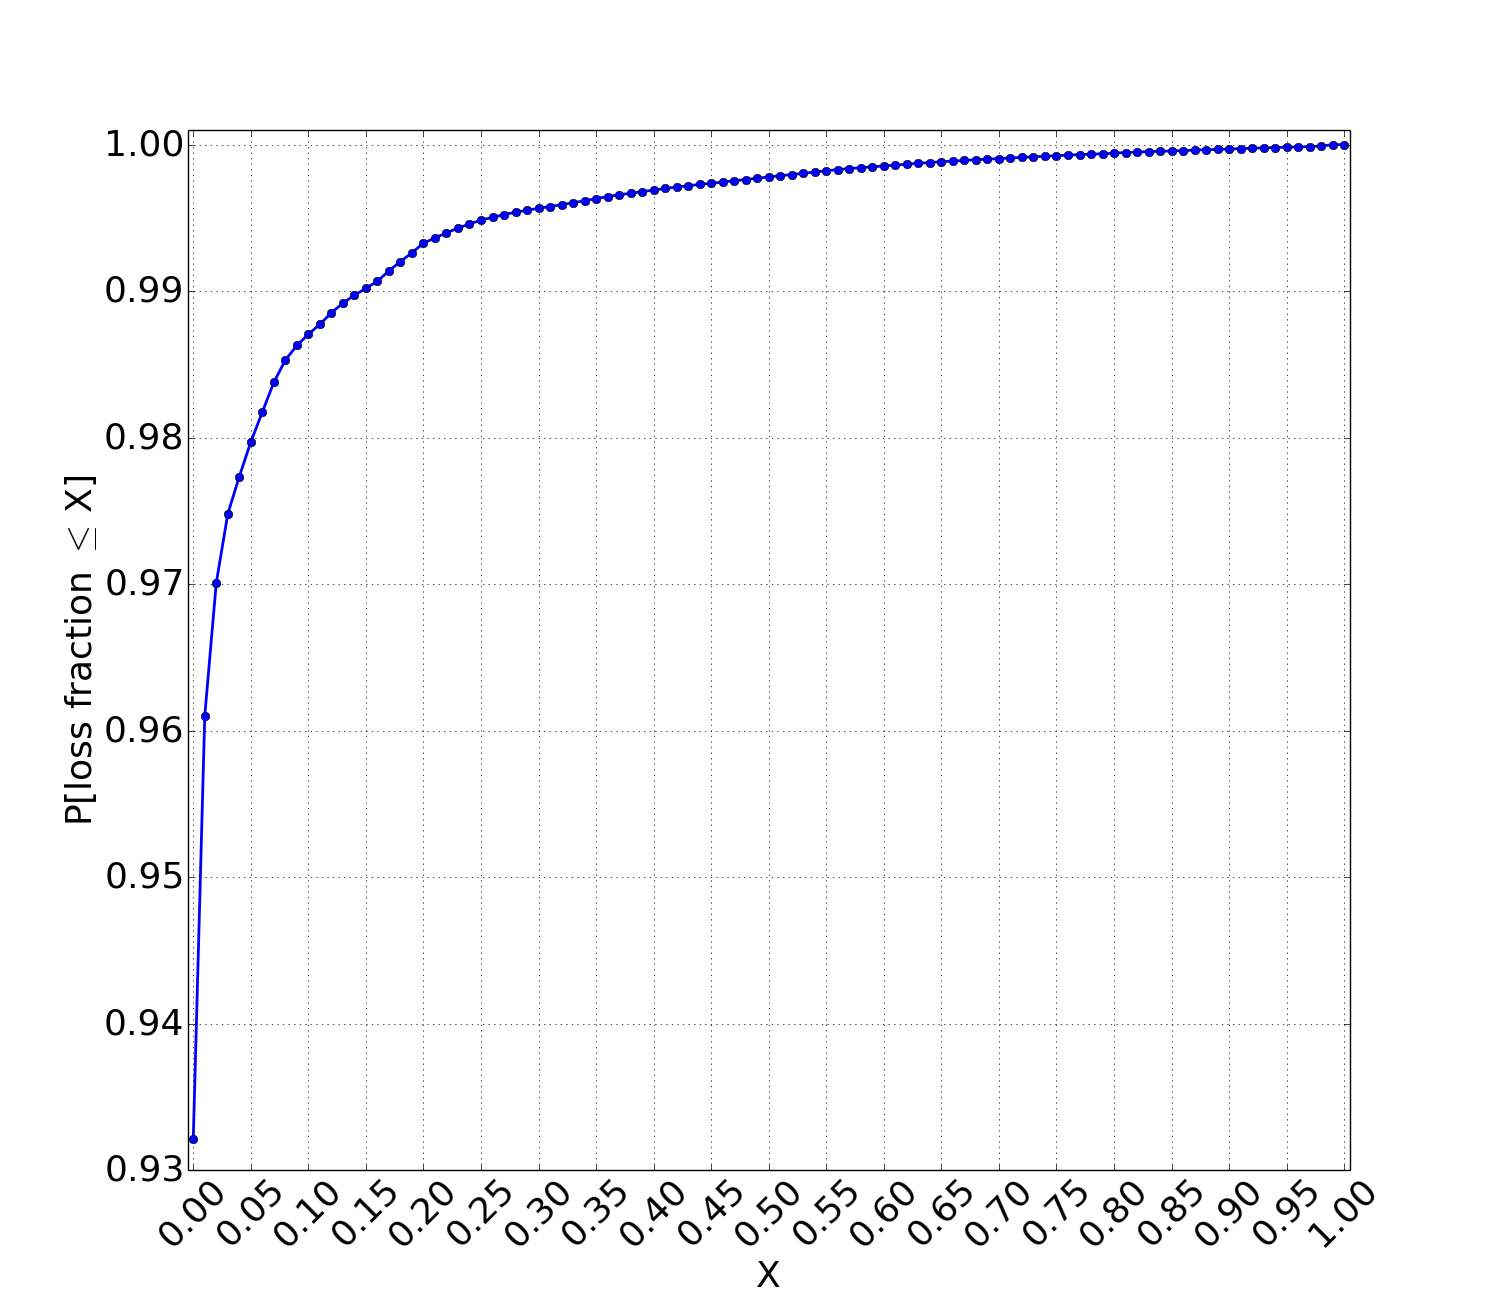
\includegraphics[width=\linewidth]{./figures/loss_cdf.png}
            \caption{CDF}
        \end{subfigure}%
        ~ 
        \begin{subfigure}[b]{0.55\textwidth}
            \centering
            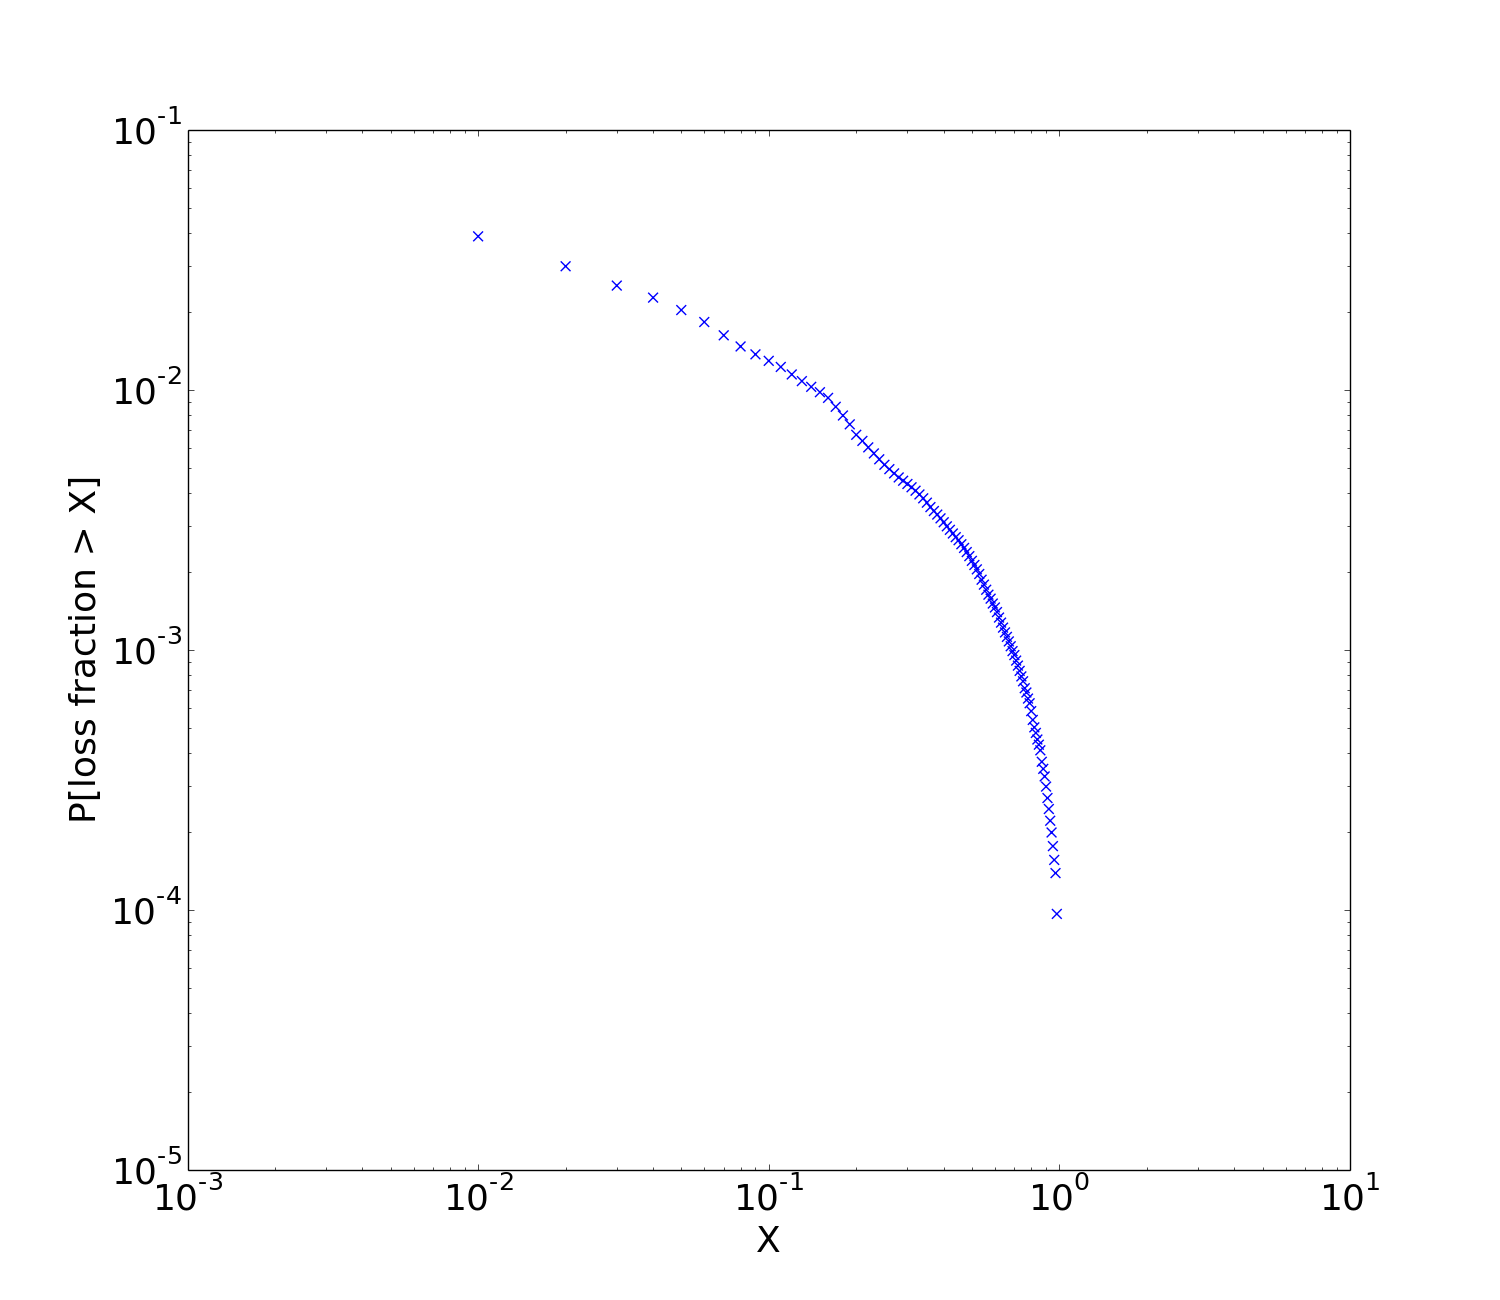
\includegraphics[width=\linewidth]{./figures/ccdf.png}
            \caption{CCDF}
        \end{subfigure}
    }
    \caption{Packet Loss Fraction}
    \label{fig:cdf_ccdf}
\end{figure}%

Figures \ref{fig:acf_ts_1}, \ref{fig:acf_ts_2}, \ref{fig:acf_ts_3} show three examples with common autocorrelation patterns in this dataset together with the time series. Since the time series are unenvely, to compute the autocorrelation function, the raw time series is transformed, and it is only considered the date and hour of a measure, ignoring the minutes and seconds. Therefore, if more than one measure occurs in the same hour, it is considered the mean.

\begin{figure}[H]
    \makebox[\linewidth][c]
    {
        %
        \centering
        \begin{subfigure}[b]{0.55\textwidth}
            \centering
            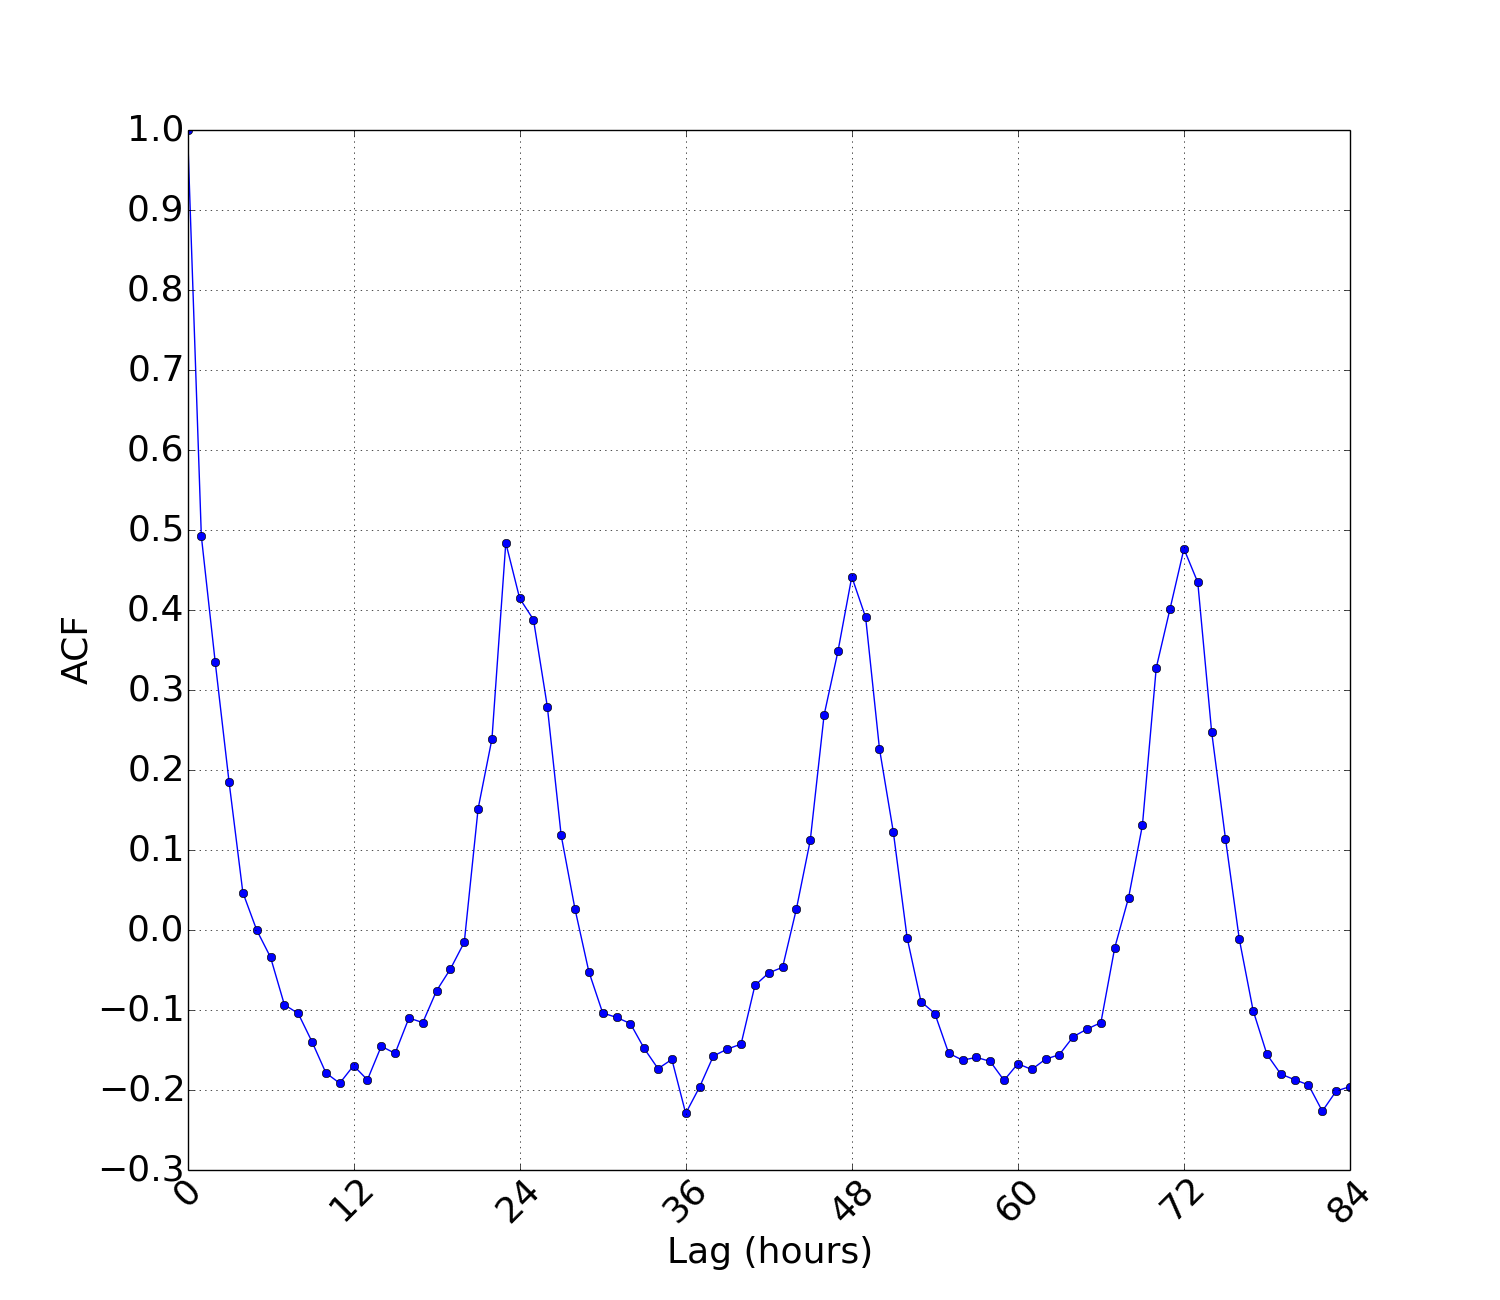
\includegraphics[width=\linewidth]{./figures/acf_NHODTCSRV04_64:66:B3:50:05:BC.png}
            \caption{Autocorrelation}
        \end{subfigure}%
        ~ 
        \begin{subfigure}[b]{0.55\textwidth}
            \centering
            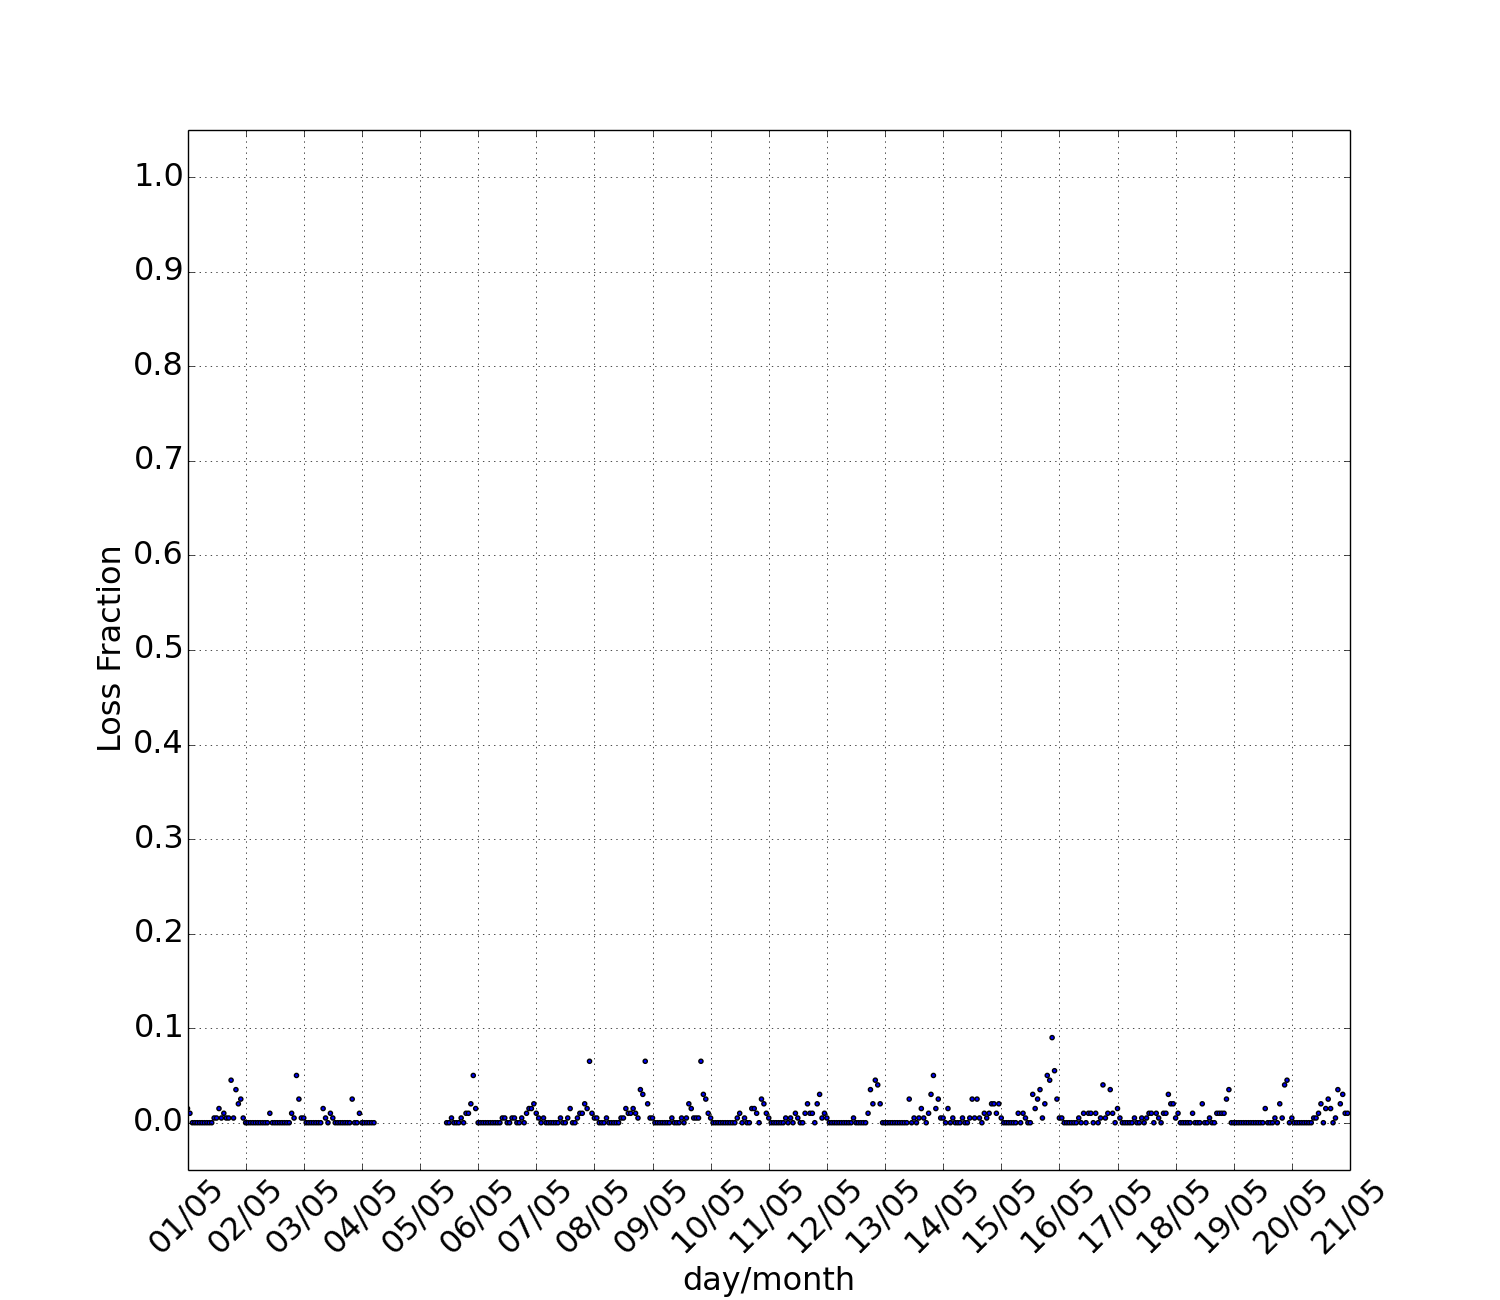
\includegraphics[width=\linewidth]{./figures/ts_NHODTCSRV04_64:66:B3:50:05:BC.png}
            \caption{Time Series}
        \end{subfigure}
    }
    \caption{Client 1}
    \label{fig:acf_ts_1}
\end{figure}%

\begin{figure}[H]
    \makebox[\linewidth][c]
    {
        %
        \centering
        \begin{subfigure}[b]{0.55\textwidth}
            \centering
            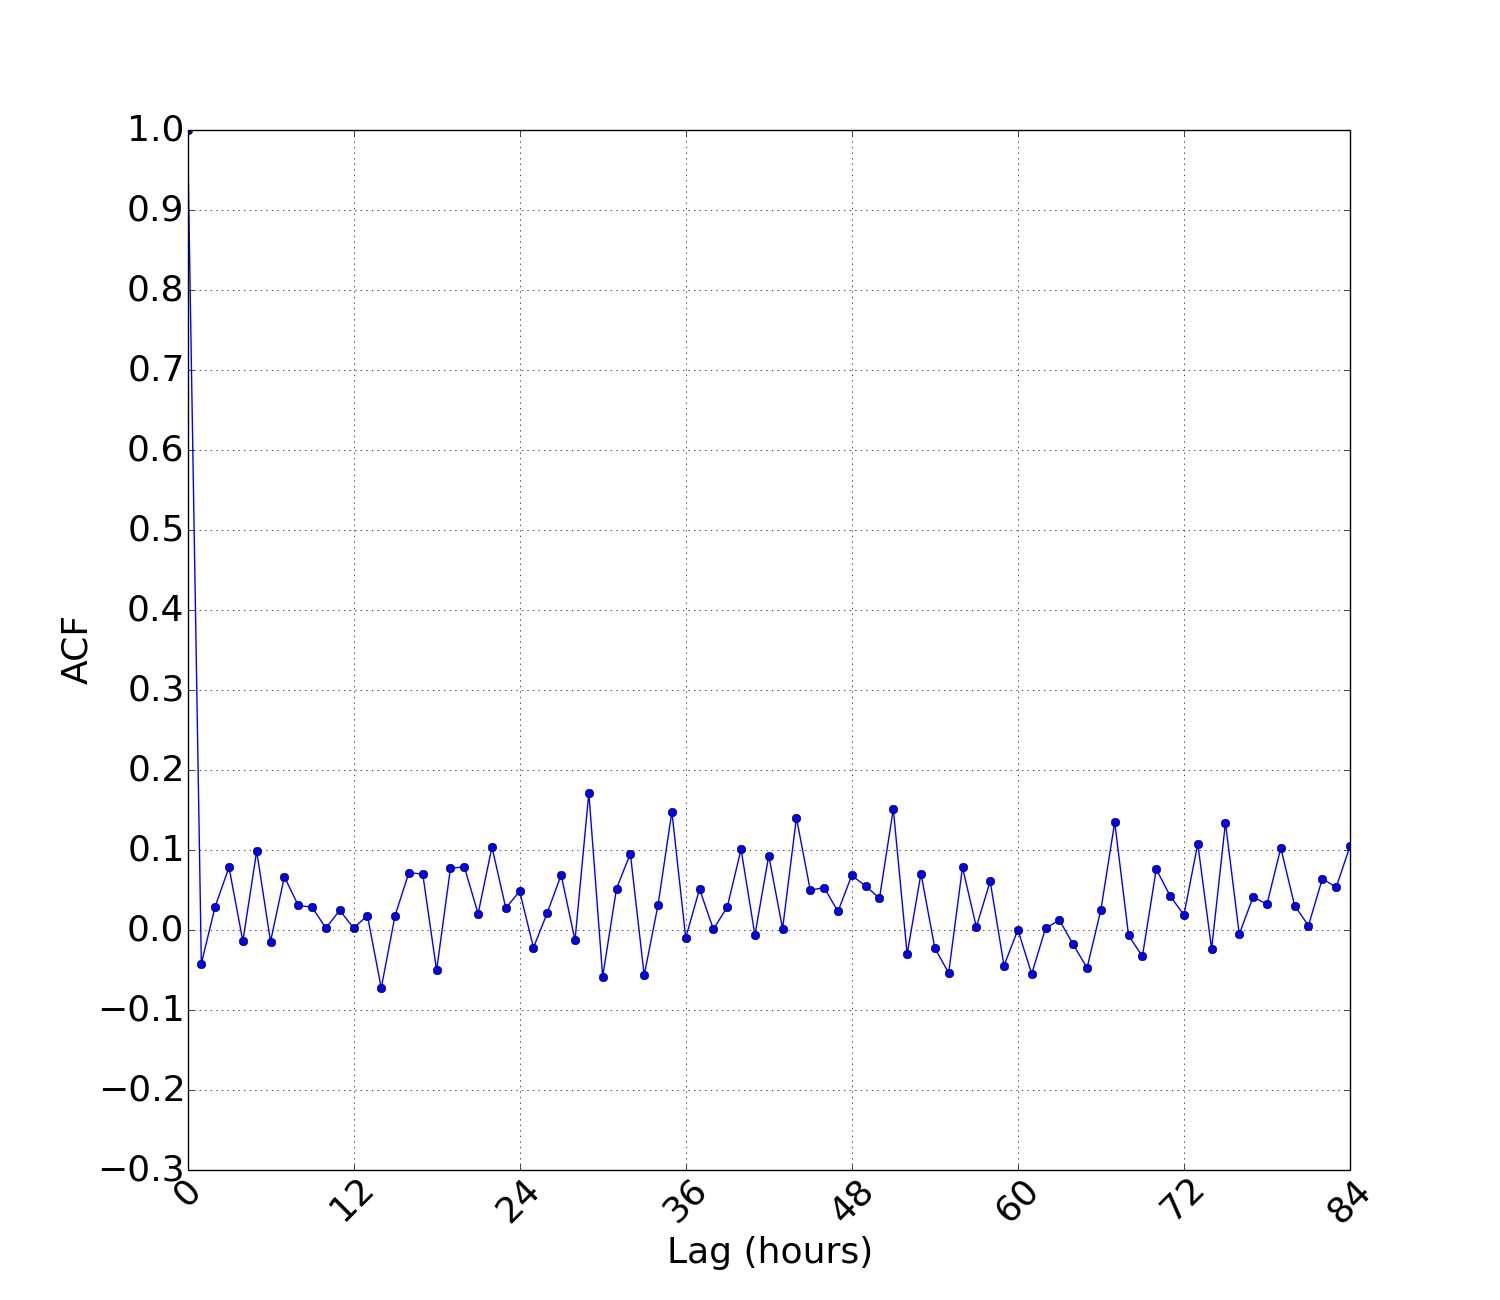
\includegraphics[width=1.0\textwidth]{./figures/acf_BREDTCSRV20_64:66:B3:7B:9E:6A.png}
            \caption{Autocorrelation}
        \end{subfigure}%
        ~ 
        \begin{subfigure}[b]{0.55\textwidth}
            \centering
            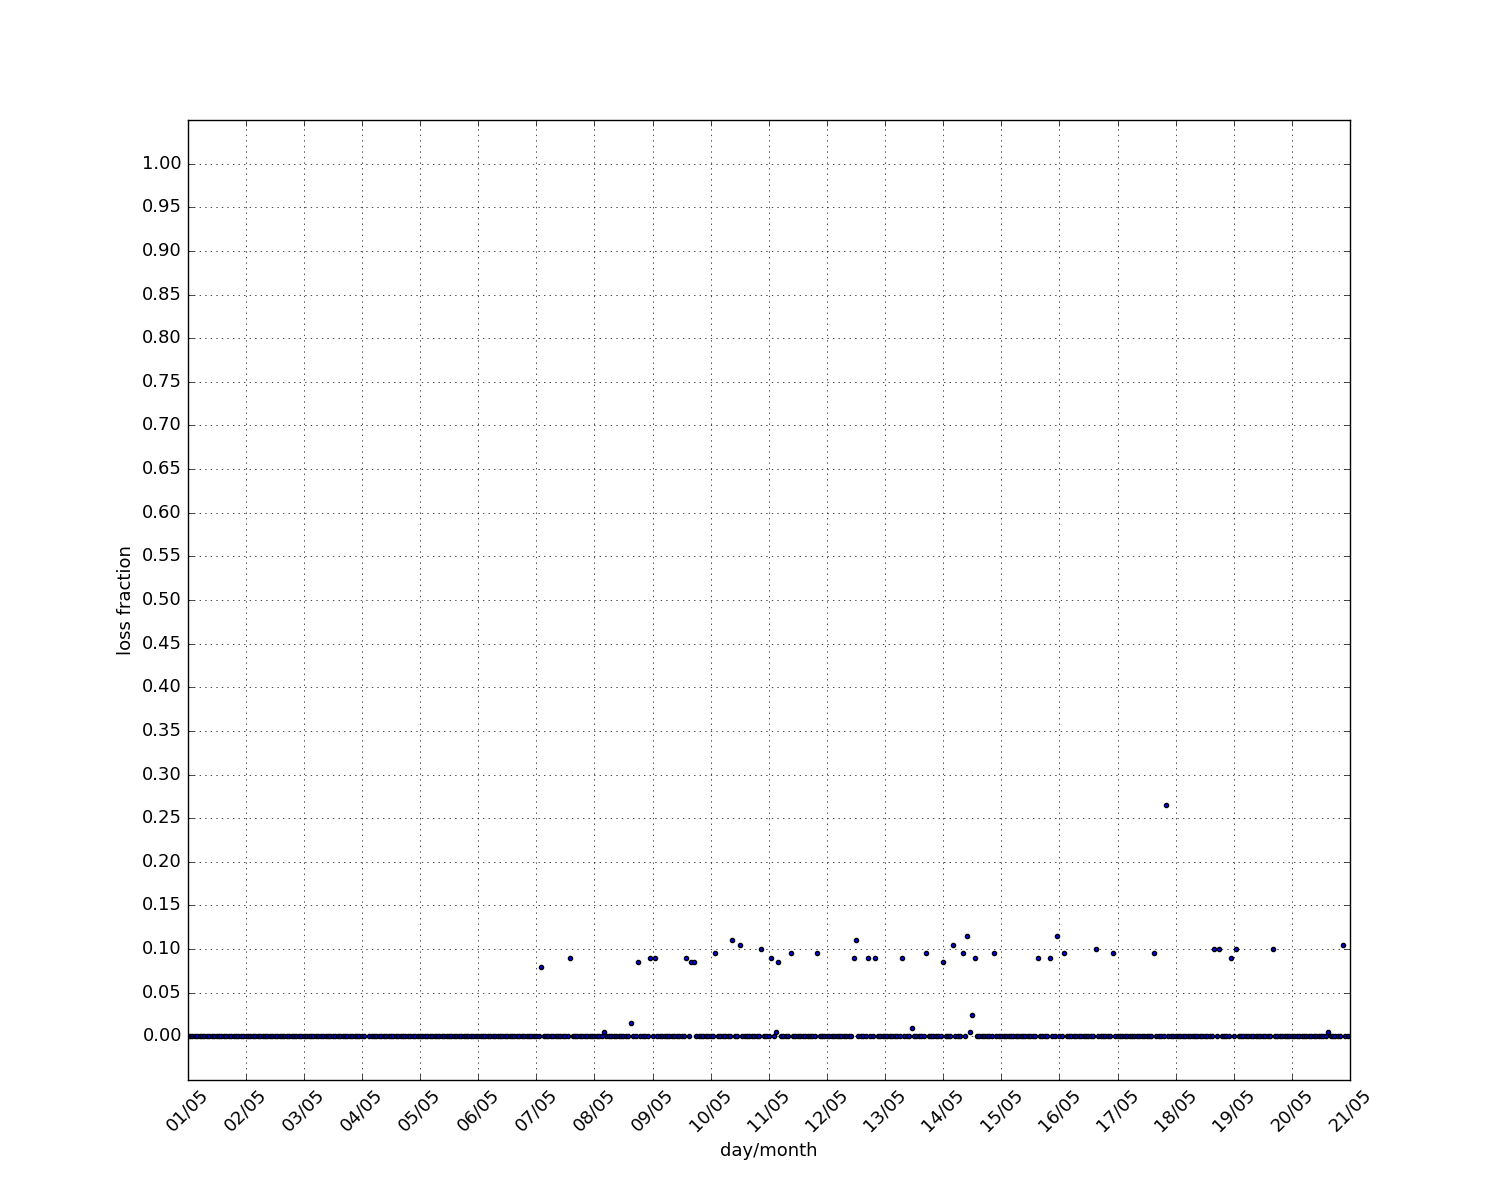
\includegraphics[width=1.0\textwidth]{./figures/ts_BREDTCSRV20_64:66:B3:7B:9E:6A.png}
            \caption{Time Series}
        \end{subfigure}
    }
    \caption{Client 2}
    \label{fig:acf_ts_2}
\end{figure}

\begin{figure}[H]
    \makebox[\linewidth][c]
    {
        %
        \centering
        \begin{subfigure}[b]{0.55\textwidth}
            \centering
            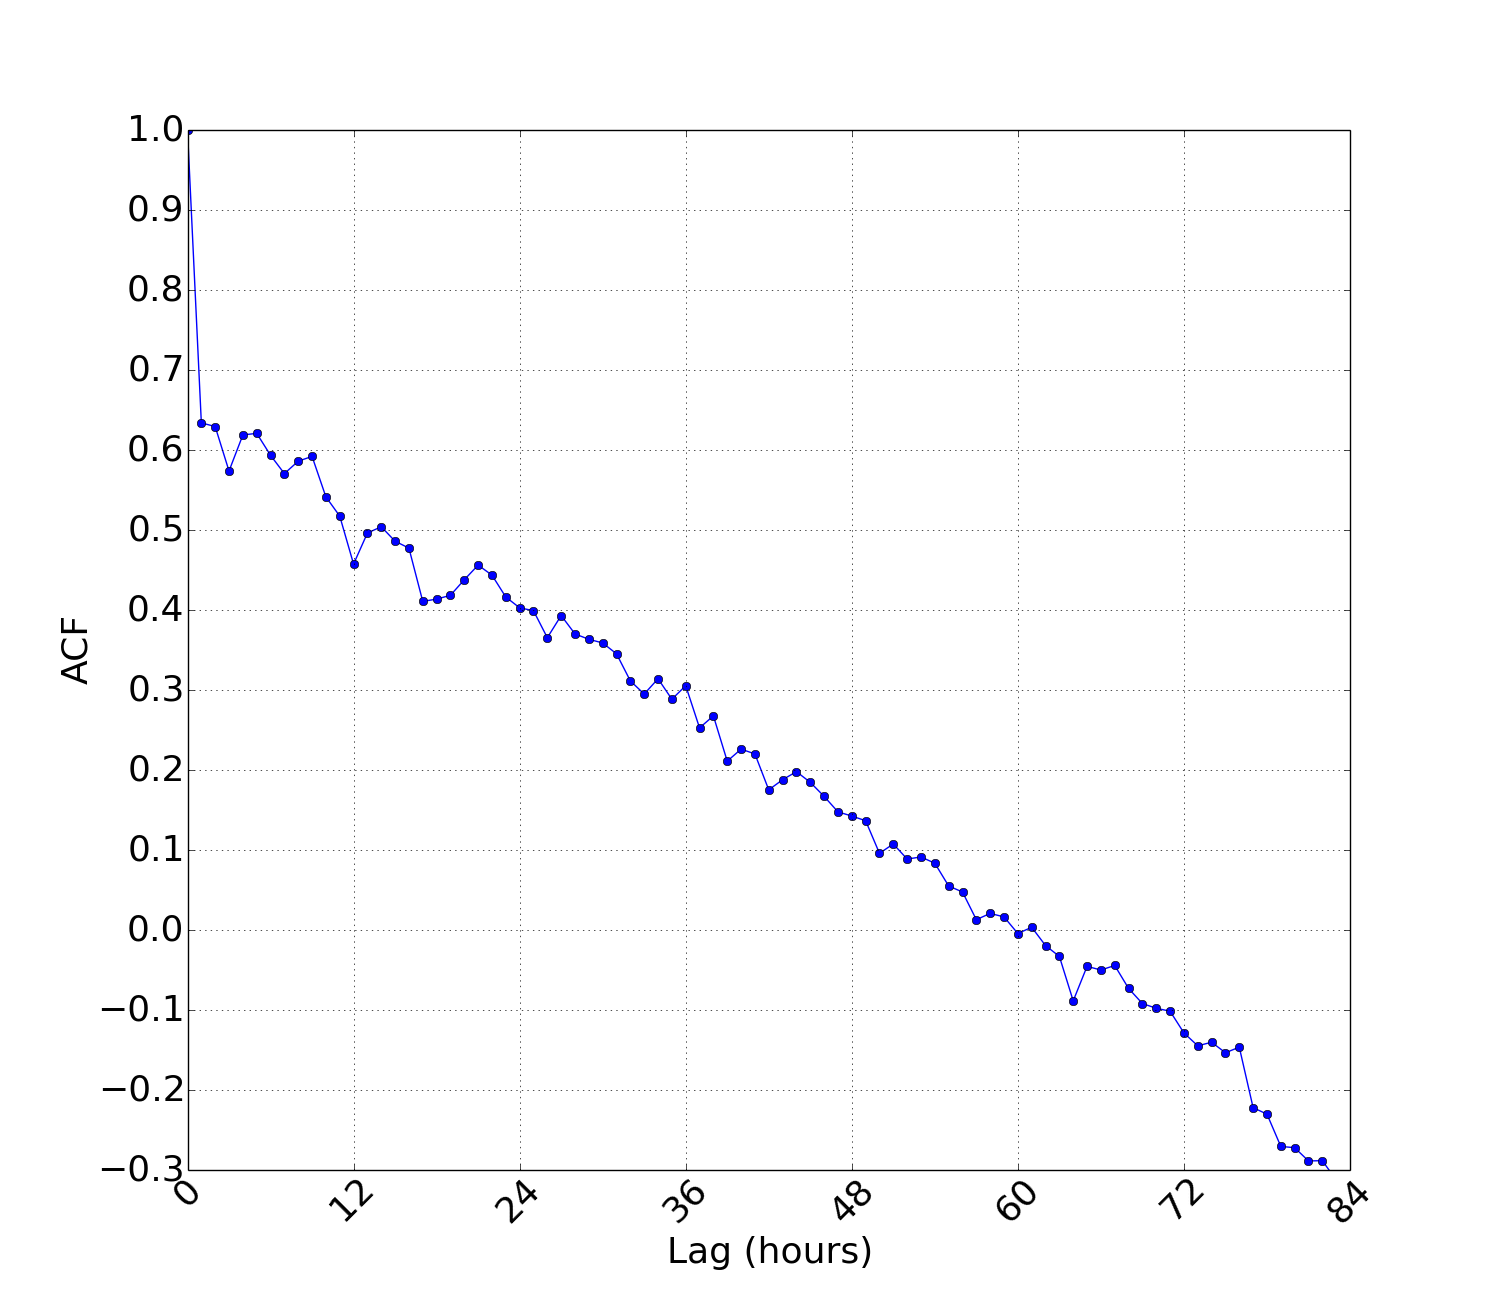
\includegraphics[width=1.0\textwidth]{./figures/acf_BHZRENPEV01_64:66:B3:A6:BA:54.png}
            \caption{Autocorrelation}
        \end{subfigure}%
        ~ 
        \begin{subfigure}[b]{0.55\textwidth}
            \centering
            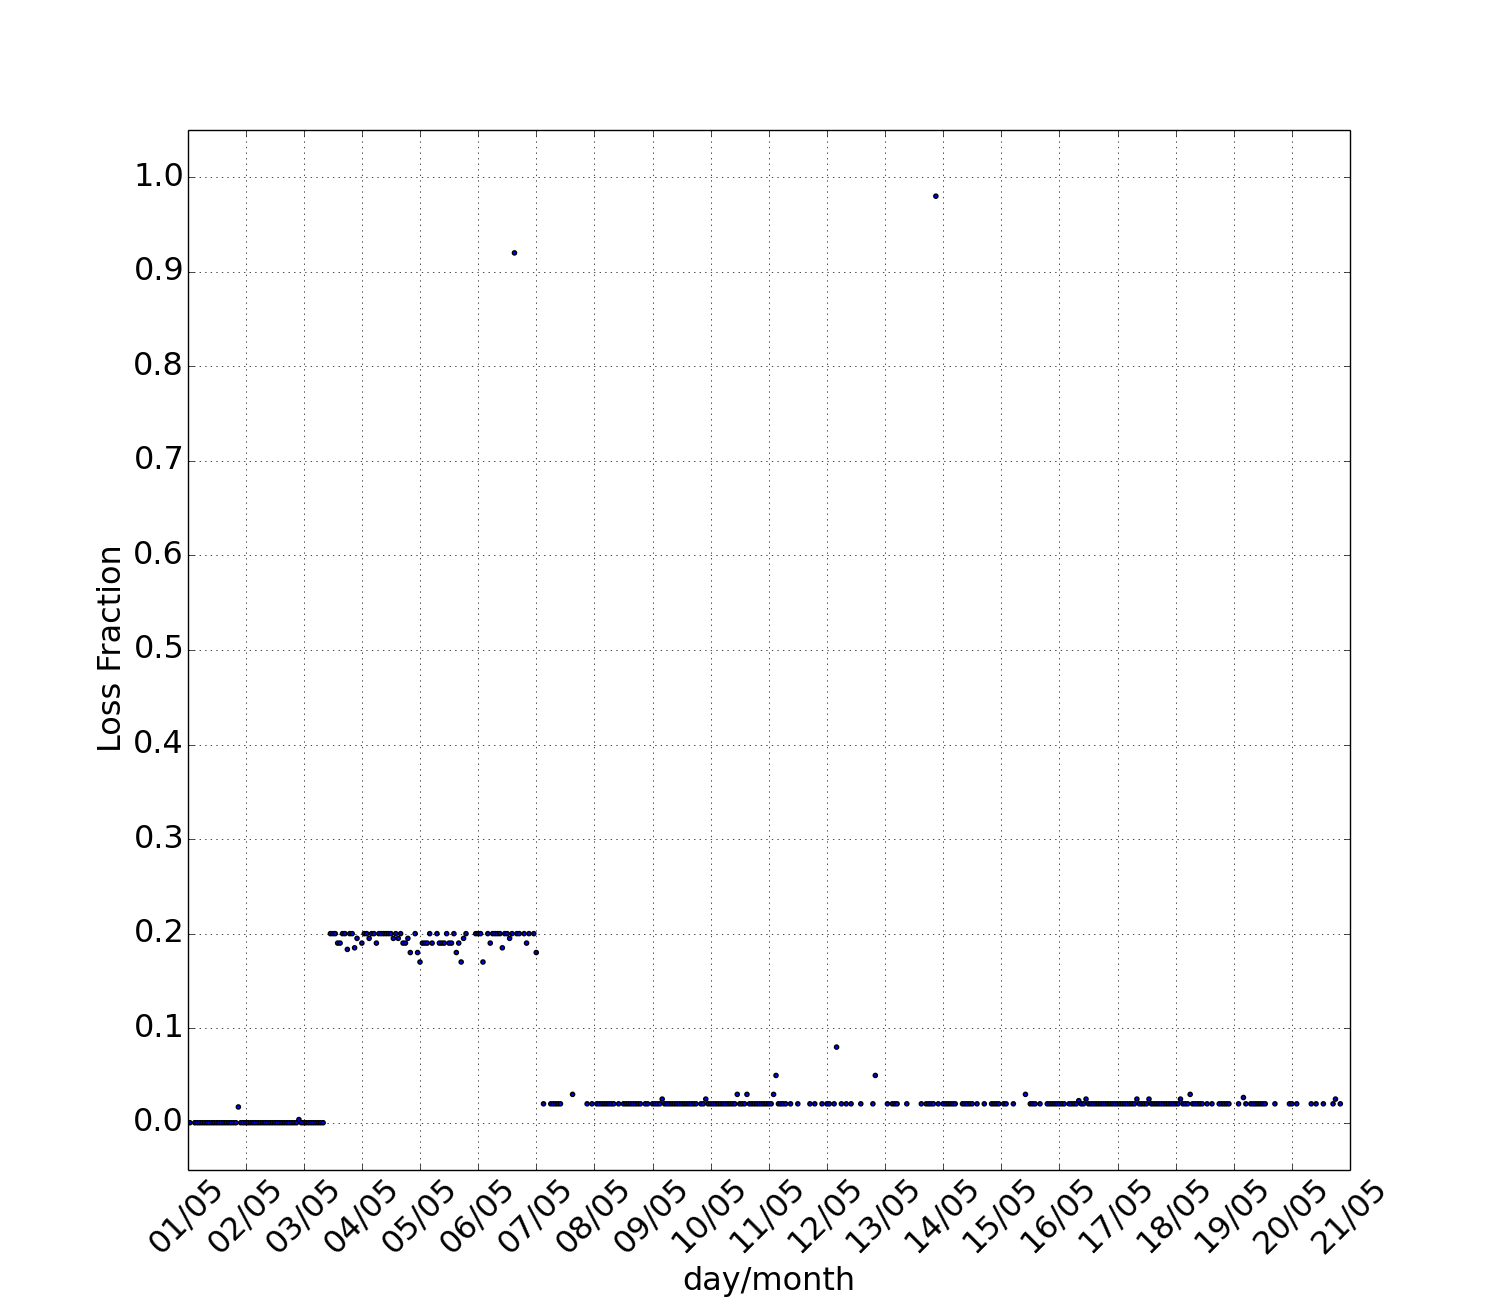
\includegraphics[width=1.0\textwidth]{./figures/ts_BHZRENPEV01_64:66:B3:A6:BA:54.png}
            \caption{Time Series}
        \end{subfigure}
    }
    \caption{Client 3}
    \label{fig:acf_ts_3}
\end{figure}

The autocorrelation of figure~\ref{fig:acf_ts_1} have a periodic pattern, with peaks in multiple of 24 hours. In this client, it is possible to observe that losses a more frequent in the end of the day. However, in figure~\ref{fig:acf_ts_2} the autocorrelation quickly decreases and fluctuates around zero. The correspondent time series have a commmon characteristics, until day 06 of may there no measures with losses, however, from then on frequently measures with losses alternated with zero losses measures. Figure~\ref{fig:acf_ts_3} shows an linear decreasing autocorrelation, and the associated time series, which presents abrupts change in the mean. 

Also, through a visual analysis, as in the previuous figures, is possible to observer diverse time series patterns and change point patterns.

As in figure~\ref{fig:acf_ts_1} same clients have a daily pattern in which losses occur more frequently at night, in which the Internet usage is known to be bigger. Figure~\ref{fig:mean_day_hour_ts} corroborates that observation, which presents the mean and variance of the measures that occurred in a specific hour during the 20 days period. This can be a indication of congestion during peak of usage hours.

\begin{figure}[H]
    \makebox[\linewidth][c]
    {
        %
        \centering
        \begin{subfigure}[b]{0.55\textwidth}
            \centering
            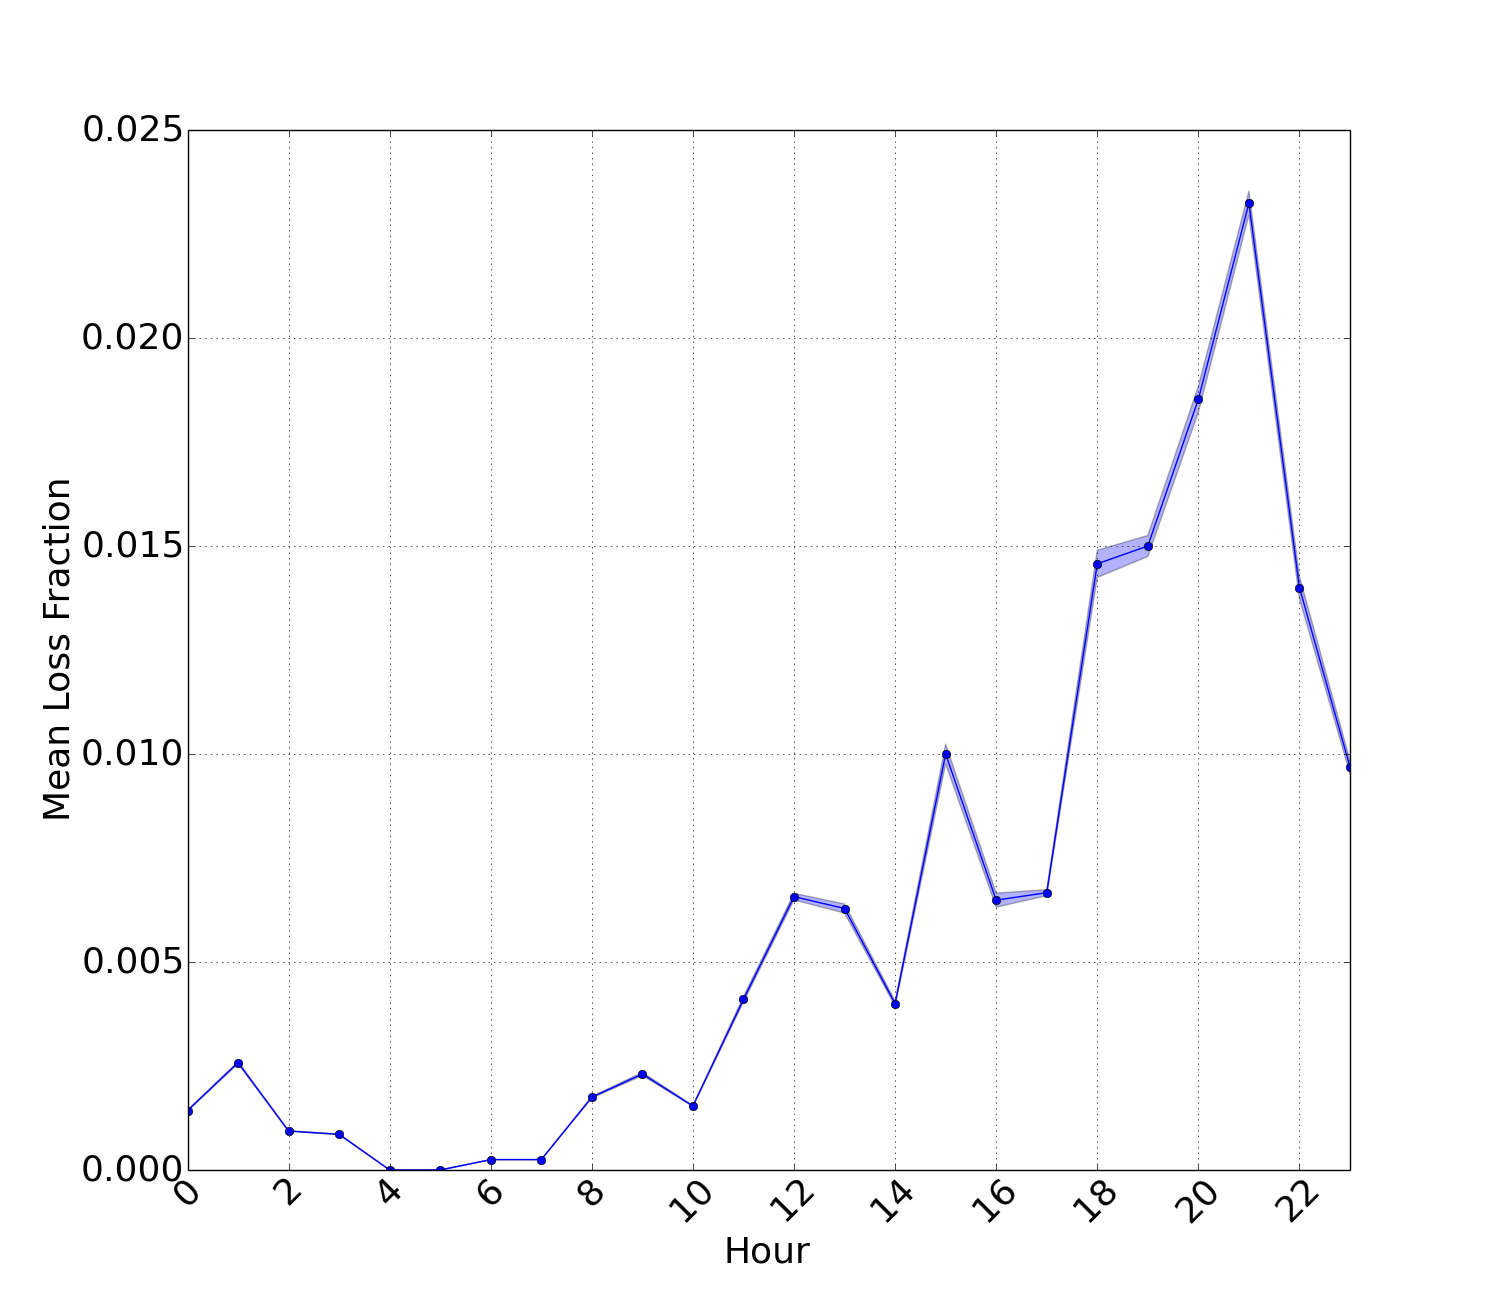
\includegraphics[width=1.0\textwidth]{./figures/mean_per_hour_in_a_day_NHODTCSRV04_64:66:B3:50:06:90.png}
            \caption{Mean and variance per hour}
        \end{subfigure}%
        ~ 
        \begin{subfigure}[b]{0.55\textwidth}
            \centering
            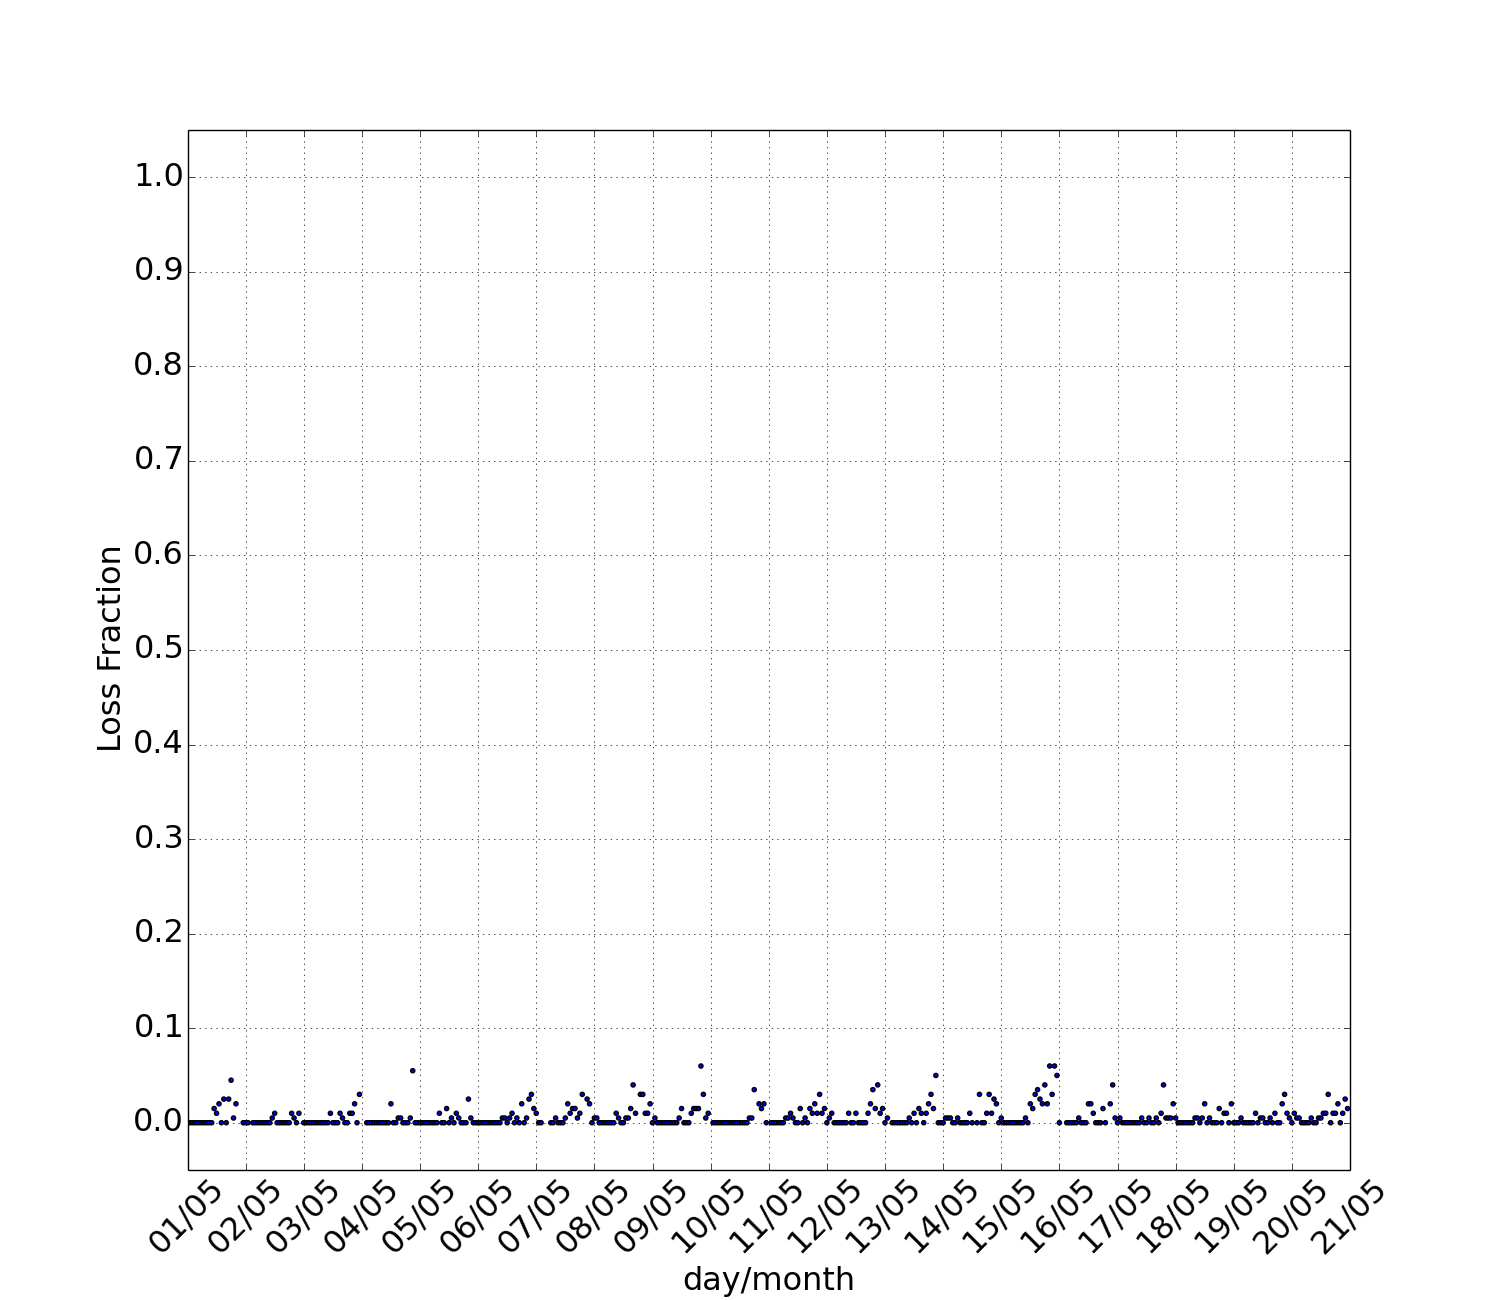
\includegraphics[width=1.0\textwidth]{./figures/ts_NHODTCSRV04_64:66:B3:50:06:90.png}
            \caption{Time Series}
        \end{subfigure}
    }
    \caption{Client 1}
    \label{fig:mean_day_hour_ts}
\end{figure}

% - mean loss by week day of single client\\
% - power spectra to check periodicity? \\

\section{Change Points Dataset}

There are several approaches to construct a change points dataset to test a change point detection method. Some works in the literature simply create a simulated time series thorugh generative models, however different segments are generated by the same model but with different parameters. In general, this types of time series are more easily handled in change point detection algorithms, since some methods assumes the same models that generated the data or because real data can have more complex characteristics. Another way is to create a time series appending different segments provenient from different real time series data. In this cases is easy to simplify the dataset since some characteristics as the segments lengths are defined by the dataset creator and another ones are fakely introduced. Another works assumes that the latent information of the time series are available, and with specific knowledge of the application field, it is possible to assume what kinds of configuration changes could induce a change in the time series. In the case of the application field of the present work this would be difficult, since the latent information would be connected with the network situation such as network topology, characteristics of routers congestions, physical equipments problems, which is a too complex, or even impossible information to collect and also to assume which variables could impact the time series. Other apprach also uses the latent information but instead creates a controlled environment in which is possible to change the configuration over time, but as in the previous case, this would be too complex. The approach followed by this work was to use a visual annotation of the time series. It were conducted, with an application domain specialist, visuallyu indicating the relevant changes. It is known that human visual inspection methods can bring erroneous conclusions, but with the data and application scenarion it was the best fit, as network engineers visually identify, after simple automatic filters, the change points.

This work is interested in work directly with real data and satisfy a real application problem.

As in other tasks, it is difficult to translate a human visual perception in a sistematically method.

In general, when the exact types of target changes are previously know the problem is easier.

\section{Methodology}

It was created an annotation system to a specialist visually indicates the change points of the time series dataset. The user indicated with the mouse the points in time where he thinks that where the cahnge points occurred. To avoid results misunderstanding X axis of the time series represented onlu the time order of the measures, since the time series are unevenly this fact could visually wrong infer change points. Also, since is known that variances in the losses fractions when the losses are low have more impact in the user QoE than when the losses are big, the system also provides two other y scales than linear, the log scale and piecewise linear with bigger length in [0, 0.1] than (0.1, 1.0]. The user can click in any scale.

A single person classified all time series. This person has experiences with academic and industry network measurements and statistical modelling, however without background in change point detection analysis. The user could take the time he wants to make a classification and it was able to classify in different days. Before the user could start the classifications, it was indicated a series of instructions: 

\begin{itemize}
    \item In the case of packet loss fraction, mean changes between 0 and 0.1 are more sensible to the end users.
    \item The "time" axis only represents the temporal order of the measurements. However, in general, consecutive points in "time" axis are separated by 30 minutes.
    \item Outlier is not a statistical change. An outlier is an observation that lies outside the overall pattern of a distribution.
\end{itemize}

Since several time series of the previously described time series have almost all measures with zero losses, these time series was filtered to reduce the number of time series and keep only the ones which provide change points, increasing the entropy. Also, to better the visualization, it was selected time with 10 days of data, therefore the dataset consists of time series from 1 may 2016 to 10 may 2016, and from 11 may 2016 to 20 may 2016. The specific filter was: it was selected only the time series that has 85\% of the maximum possible data in the specified time period, considering that each home router executes the measurement procedure at most two times in a hour. Reducing to 522 time series. Also it were only selected the time series that have at least one window of length 48 with at least 6 measures with loss fraction bigger than 0.01.

\section{Descriptive Analysis}

- explain possible ways to get the ground truth\\
- description of the volunteer\\
- user instructions\\
- snapshots of system\\ 
- how time series were selected to be in the survey\\

\section{Description of Change Points Dataset}

- number of time series, number of change points: it is a high dimensional problem\\
- distribution number of changes per time series\\
- distribution time between change points\\
- distribution time for the first change point\\
- distribution time from last change point to time series end\\
- distribution of classification time?\\
- measure the difference between consecutive segments?\\

\section{Performance Evaluation}

- how the performance is asserted in literature\\
- ROC curve\\
- confusion matrix and accuracy metrics\\

    \chapter{Conclusions}
\label{chap:conclusion}

Considering the specific \gls*{isp}'s topology, and the current end-to-end measurement
methodology, this dissertation proposes a data analytics framework to
detect and localize network events.
For such purpose, the mechanism tracks
statistical changes in the end-to-end \gls*{qos} time series from different clients,
and correlates these patterns with traceroutes.
Finally, several outcomes were presented when the procedure was applied to
real data.

The results show that, considering the exposed restrictions,
it is possible to use only end-to-end \gls*{qos} metrics, and traceroutes, from
different clients, to identify and localize network events.
However, due to the lack of an events dataset ground truth, important
questions persist unanswered.
For instance, a quantitative accuracy study
would allow to check which types of events can't be handled by the
proposed mechanism.
A dataset would also allow a precise analysis of the events
patterns, how they impact the \gls*{qos} metrics, and fine tune the system.

The use of end-to-end measurements has the advantage of dealing with
metrics that are directly related with the service perceived by the customers.
As an example, this feature can be used to rank simultaneous failure events
according with their impact to the end-users.
Nonetheless, would be interesting to study the impact of introducing
internal network information to the framework.

Besides the data availability, the current measurement process imposed
several restrictions to this work.
In order to better explore the proposed solution,
a further continuation of this project
would require a stronger partnership with the \gls*{isp}.
In addition, in order to improve the proposed framework's performance,
it would be desirable to adapt the measurement software.
However, this dissertation can be used as a first guide to the \gls*{isp}'s engineers.

\section{Contributions}
Next is summarized this dissertation contributions.

\begin{itemize}
\item
An automatic procedure, that only uses the available end-to-end \gls*{qos}
measurements, and traceroutes, to detect and localize network events in the
specific tier-3 ISP's infrastructure.

\item
A list of possible improvements in the measurement methodology currently
employed by the startup, in order to enhance the proposed system's performance. This
list is presented in the next Section~\ref{sec:future_work}.
\end{itemize}

\section{Future Work}
\label{sec:future_work}

Next is presented a list of future development directions of this work.
Considering the detection and localization of events, several adaptations to
the current measurement methodology are suggested.

\begin{itemize}
\item
The used \gls*{qos} metrics are affected by equipments in the path from the server to
the end-user, as well as those in the reverse direction.
However, only the path information from end-users to servers are available.
Hence, the traceroutes from servers to end-users should also be collected.
Besides, instead of only considering the round trip loss information,
the one way loss fraction in both directions can be tracked.
Further, the maximum achievable one way throughput measurement can be
implemented using \gls*{udp} instead of \gls*{tcp}, which eliminates the interference of
performance degradation in the reverse path.

\item
The \gls*{hfc} plant between the home router and the
first hop of the traceroute can be incorporated to the analysis.
Also, in addition to only using end-to-end \gls*{qos} metrics,
the proposed mechanism can be extended
to use internal network devices information, such as signal-to-noise ratio.

\item
A network failure events dataset can be built with \gls*{isp}'s data.
As an example, customers' complaints gathered from call centers can be used to,
during a specific time period, infer clients affected by a \gls*{qoe} deterioration,
which can then be translated to true network failures.
Additionally, it is possible to use records from current failure detection
methods deployed by the \gls*{isp}, such as manual inspection, or through equipments
that are able to report specific faults.
However, through preliminary talks with \gls*{isp}'s engineers,
both databases are noisy, and mining useful information
from them can be a challenging task.
For instance, there are cases in which devices flaws are manually
detected and corrected, but those information is not stored.
Also, during the dataset construction, the inferred events times can be
considerably different from their true occurrence time.
As stated in Chapter~\ref{chap:methodology}, a dataset could open new
supervised learning possibilities to the change point detection problem, such
as hyperparameter optimization and model selection.
Besides, since the tier-2 \gls*{isp} is not a project partner, this
complete data of the network infrastructure may not be available.

\item
Once a network events dataset is constructed, the correlation between
change points of different \gls*{qos} metrics can reveal useful information
about the network behavior. This analysis was not done since the algorithms'
hyperparameters couldn't be optimized, hence, these comparisons could reach
wrong conclusions.

\item
A deeper knowledge of the tier-2 \gls*{isp}'s infrastructure
can be used to model the tier-2 network with finer granularity in the Spatial
Correlation procedure, which can improve the system's event localization
precision.

\item
It is planned in the \gls*{isp}'s roadmap to increase the number of tracked customers.
In this case, the system's computational performance can benefit from data
aggregation techniques, as it was done in Argus.
Besides, this increase will naturally improve the internal network equipments
coverage by the end-to-end measurements, which, as the previous topic, can
enhance the events localization precision.

\item
Once the system is deployed, the algorithms and parameters can be selected
through a reinforcement learning approach. If network operators
feedback the outcomes' correctness, the system can adaptively optimize the used
strategies.

\item
Considering a real time processing environment, in order to decrease the
event detection delay, the system can adaptively control the measurement
frequency.
Increasing the amount of data related to potentially problematic regions,
can improve the system's output confidence in a short time period.
Also, it is possible to reduce the measurement frequency in well behaved
localities, which can lower the traffic overhead generated by measurements, and
increase the data analytics computational performance.

\item
Instead of centrally process the time series,
it is possible to instrument the home
gateways to detect changes in an online fashion. Then, as with \gls*{cem}, the home
routers could push this information to a central database for further analysis.

\item
Extend the mechanism to deal with other types of network infrastructures.

\end{itemize}

    
    \backmatter
    \bibliographystyle{coppe-unsrt}
    \bibliography{./src/bibliography}

\end{document}
